% Quantitative measure of the force model (English version of quantitative_measure.tex)
% Compile: xelatex quantitative_measure_en.tex  -> ../Force_model/Quantitative measure/quantitative_measure_en.pdf
\documentclass[11pt]{article}
\usepackage[a4paper,margin=2.5cm]{geometry}
\usepackage{amsmath,amssymb}
\usepackage{tikz}
\usetikzlibrary{arrows.meta}
\setlength{\parindent}{0pt}

% Typography: vectors and matrices upright bold (\mathbf), scalars italic, not bold.
% Norms are written without the subscript 2.
\newcommand{\rh}{\hat{\mathbf{r}}}
\newcommand{\xa}{\hat{\mathbf{x}}_a}
\newcommand{\ya}{\hat{\mathbf{y}}_a}
\newcommand{\za}{\hat{\mathbf{z}}_a}
\newcommand{\Ij}{\mathbf{I}}
\newcommand{\Ijh}{\hat{\mathbf{I}}}
\newcommand{\fij}{\mathbf{f}_{i}}

\begin{document}

\begin{center}
{\LARGE\bfseries Quantitative measure of the force model}
\end{center}
\vspace{6pt}

% ---------------------------------------------------------------------------------------
\section*{Step 1}

\subsection*{1.1\ \ Unit direction $\rh(\varphi,\theta)$}

An arbitrary unit direction $\rh$ is described in the actuator-frame basis $\{\xa,\ \ya,\ \za\}$:

\begin{minipage}[c]{0.54\textwidth}
\[
\rh(\varphi,\theta)
=\cos\varphi\cos\theta\,\xa+\cos\varphi\sin\theta\,\ya+\sin\varphi\,\za
=\begin{bmatrix}
\cos\varphi\cos\theta\\
\cos\varphi\sin\theta\\
\sin\varphi
\end{bmatrix}
\]
\[
\left\{
\begin{aligned}
\varphi &\in [-90^\circ,\ 90^\circ] &&\text{elevation (from the $x_a$--$y_a$ plane)}\\
\theta  &\in [0^\circ,\ 360^\circ)  &&\text{azimuth (from the $+x_a$ axis, about $z_a$)}
\end{aligned}\right.
\]
\[
\|\rh\|=1
\]
\end{minipage}
\hfill
\begin{minipage}[c]{0.42\textwidth}
\centering
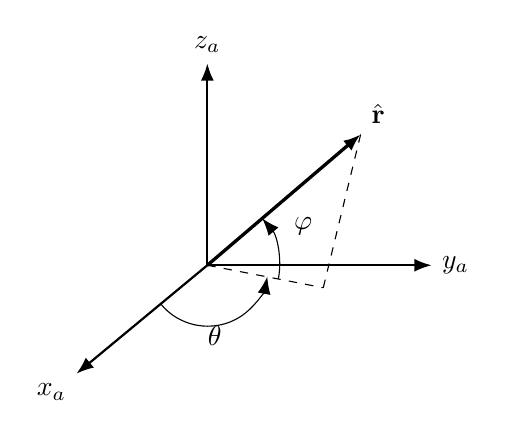
\begin{tikzpicture}[scale=0.95,>={Latex[length=2.2mm]}]
  \coordinate (O) at (0,0);
  \draw[->,thick] (O) -- (0,2.7)        node[above]{$z_a$};
  \draw[->,thick] (O) -- (3.0,0)        node[right]{$y_a$};
  \draw[->,thick] (O) -- (-1.75,-1.45)  node[below left]{$x_a$};
  \coordinate (V) at (2.05,1.75);
  \coordinate (Q) at (1.55,-0.30);
  \draw[->,very thick] (O) -- (V) node[above right]{$\rh$};
  \draw[dashed] (O) -- (Q);
  \draw[dashed] (Q) -- (V);
  \draw[->] (0.95,-0.18) arc (-10.5:40.5:0.97);
  \node at (1.28,0.52) {$\varphi$};
  \draw[->] (-0.62,-0.52) arc (219.5:349.5:0.81);
  \node at (0.10,-0.95) {$\theta$};
\end{tikzpicture}
\end{minipage}

\subsection*{1.2\ \ Current $\Ij$}

The force vector produced at position $\mathbf{p}_i$ by the current $\Ij$:
\[
\fij=\begin{bmatrix} f_{i1}\\ f_{i2}\\ f_{i3} \end{bmatrix},\qquad
f_{ik}=\Ij^{\mathsf T}\,{}^{F}\hat{\mathbf{H}}_{I}^{\mathsf T}\,
\mathbf{L}_k\!\left(\mathbf{p}_i/\hat{\ell},\,\hat{\mathbf{e}}\right)\,{}^{F}\hat{\mathbf{H}}_{I}\,\Ij,
\qquad k=1,2,3
\]
Let
\[
\Ij=\sqrt{\|\fij\|}\;\Ijh,\qquad
\mathbf{f}\!\left(\mathbf{p}_i,\Ij\right)=\|\fij\|\,\rh
\]
Substituting into the force model:
\[
\begin{aligned}
\fij
&=\begin{bmatrix}
\left(\sqrt{\|\fij\|}\,\Ijh\right)^{\!\mathsf T}{}^{F}\hat{\mathbf{H}}_{I}^{\mathsf T}\,\mathbf{L}_1\!\left(\mathbf{p}_i/\hat{\ell},\hat{\mathbf{e}}\right){}^{F}\hat{\mathbf{H}}_{I}\left(\sqrt{\|\fij\|}\,\Ijh\right)\\[2pt]
\left(\sqrt{\|\fij\|}\,\Ijh\right)^{\!\mathsf T}{}^{F}\hat{\mathbf{H}}_{I}^{\mathsf T}\,\mathbf{L}_2\!\left(\mathbf{p}_i/\hat{\ell},\hat{\mathbf{e}}\right){}^{F}\hat{\mathbf{H}}_{I}\left(\sqrt{\|\fij\|}\,\Ijh\right)\\[2pt]
\left(\sqrt{\|\fij\|}\,\Ijh\right)^{\!\mathsf T}{}^{F}\hat{\mathbf{H}}_{I}^{\mathsf T}\,\mathbf{L}_3\!\left(\mathbf{p}_i/\hat{\ell},\hat{\mathbf{e}}\right){}^{F}\hat{\mathbf{H}}_{I}\left(\sqrt{\|\fij\|}\,\Ijh\right)
\end{bmatrix}\\[6pt]
&=\|\fij\|
\begin{bmatrix}
\Ijh^{\mathsf T}\,{}^{F}\hat{\mathbf{H}}_{I}^{\mathsf T}\,\mathbf{L}_1\!\left(\mathbf{p}_i/\hat{\ell},\hat{\mathbf{e}}\right){}^{F}\hat{\mathbf{H}}_{I}\,\Ijh\\[2pt]
\Ijh^{\mathsf T}\,{}^{F}\hat{\mathbf{H}}_{I}^{\mathsf T}\,\mathbf{L}_2\!\left(\mathbf{p}_i/\hat{\ell},\hat{\mathbf{e}}\right){}^{F}\hat{\mathbf{H}}_{I}\,\Ijh\\[2pt]
\Ijh^{\mathsf T}\,{}^{F}\hat{\mathbf{H}}_{I}^{\mathsf T}\,\mathbf{L}_3\!\left(\mathbf{p}_i/\hat{\ell},\hat{\mathbf{e}}\right){}^{F}\hat{\mathbf{H}}_{I}\,\Ijh
\end{bmatrix}\\[6pt]
&=\|\fij\|\;\hat{\mathbf{f}}\!\left(\mathbf{p}_i,\Ijh\right)
\end{aligned}
\]
Comparing the two gives
\[
\hat{\mathbf{f}}\!\left(\mathbf{p}_i,\Ijh\right)=\rh
\]
$\hat{\mathbf{f}}(\mathbf{p}_i,\Ijh)$ is called the unit force, and the corresponding current $\Ijh$ the unit current.

% ---------------------------------------------------------------------------------------
\section*{Step 2}

The desired force $\mathbf{f}_d$ is split into magnitude and direction:
\[
\mathbf{f}_d=\|\mathbf{f}_d\|\,\rh(\varphi,\theta)
\]
\[
\mathbf{I}_{\mathrm{opt}}=\arg\min_{\Ij}\ \|\Ij\|^2
\qquad\text{s.t.}\quad \mathbf{f}\!\left(\mathbf{p}_i,\Ij\right)=\mathbf{f}_d\!\left(\mathbf{p}_i,\mathbf{I}_{\mathrm{opt}}\right)
\]
Replacing $\Ij$ by $\Ij=\sqrt{\|\fij\|}\;\Ijh$:
\[
\|\Ij\|^2=\|\fij\|\,\|\Ijh\|^2,\qquad
\mathbf{f}\!\left(\mathbf{p}_i,\Ij\right)=\|\fij\|\,\hat{\mathbf{f}}\!\left(\mathbf{p}_i,\Ijh\right)=\mathbf{f}_d
\]
The constraint gives $\|\fij\|=\|\mathbf{f}_d\|$ and $\hat{\mathbf{f}}(\mathbf{p}_i,\Ijh)=\mathbf{f}_d/\|\mathbf{f}_d\|=\rh$, where $\|\mathbf{f}_d\|$ is a constant.\\[4pt]
The problem becomes the minimum-norm unit-current problem:
\[
\hat{\mathbf{I}}_{\mathrm{opt}}=\arg\min_{\Ijh}\ \|\Ijh\|^2
\qquad\text{s.t.}\quad \hat{\mathbf{f}}\!\left(\mathbf{p}_i,\Ijh\right)=\rh
\]
Solution of the original problem:
\[
\mathbf{I}_{\mathrm{opt}}=\sqrt{\|\mathbf{f}_d\|}\;\hat{\mathbf{I}}_{\mathrm{opt}}
\]

% ---------------------------------------------------------------------------------------
\section*{Step 3}

For a fixed position $\mathbf{p}_i$, $\hat{\mathbf{I}}_{\mathrm{opt}}(\mathbf{p}_i,\varphi,\theta)$ is solved for an arbitrary direction $\rh$ with Lagrange multipliers. Let
\[
\mathbf{Q}_k={}^{F}\hat{\mathbf{H}}_{I}^{\mathsf T}\,\mathbf{L}_k\!\left(\mathbf{p}_i/\hat{\ell},\hat{\mathbf{e}}\right){}^{F}\hat{\mathbf{H}}_{I},
\qquad k=1,2,3
\]
The $k$-th component of the constraint $\hat{\mathbf{f}}(\mathbf{p}_i,\Ijh)=\rh$ is $\Ijh^{\mathsf T}\mathbf{Q}_k\Ijh=r_k$;
with the Lagrange multipliers $\boldsymbol{\lambda}=\begin{bmatrix}\lambda_1 & \lambda_2 & \lambda_3\end{bmatrix}^{\mathsf T}$:
\[
\mathcal{L}\!\left(\Ijh,\boldsymbol{\lambda}\right)
=\|\Ijh\|^2-\sum_{k=1}^{3}\lambda_k\left(\Ijh^{\mathsf T}\mathbf{Q}_k\Ijh-r_k\right)
\]

% ---------------------------------------------------------------------------------------
\section*{Step 4}

With $\hat{\mathbf{I}}_{\mathrm{opt}}$ obtained from the Lagrange multipliers, the normalized current is
\[
\bar{\mathbf{I}}=\frac{\hat{\mathbf{I}}_{\mathrm{opt}}}{\left\|\hat{\mathbf{I}}_{\mathrm{opt}}\right\|},\qquad
\|\bar{\mathbf{I}}\|=1
\]
Substituting a current of magnitude $\|\mathbf{I}\|$ (A), $\mathbf{I}=\|\mathbf{I}\|\,\bar{\mathbf{I}}$, into the force model:
\[
\begin{aligned}
\mathbf{f}\!\left(\mathbf{p}_i,\mathbf{I}(\varphi,\theta)\right)
&=\|\mathbf{I}\|^2
\begin{bmatrix}
\bar{\mathbf{I}}^{\mathsf T}\mathbf{Q}_1\bar{\mathbf{I}}\\[2pt]
\bar{\mathbf{I}}^{\mathsf T}\mathbf{Q}_2\bar{\mathbf{I}}\\[2pt]
\bar{\mathbf{I}}^{\mathsf T}\mathbf{Q}_3\bar{\mathbf{I}}
\end{bmatrix}\\[6pt]
&=\frac{\|\mathbf{I}\|^2}{\left\|\hat{\mathbf{I}}_{\mathrm{opt}}\right\|^2}
\begin{bmatrix}
\hat{\mathbf{I}}_{\mathrm{opt}}^{\mathsf T}\mathbf{Q}_1\hat{\mathbf{I}}_{\mathrm{opt}}\\[2pt]
\hat{\mathbf{I}}_{\mathrm{opt}}^{\mathsf T}\mathbf{Q}_2\hat{\mathbf{I}}_{\mathrm{opt}}\\[2pt]
\hat{\mathbf{I}}_{\mathrm{opt}}^{\mathsf T}\mathbf{Q}_3\hat{\mathbf{I}}_{\mathrm{opt}}
\end{bmatrix}
=\frac{\|\mathbf{I}\|^2}{\left\|\hat{\mathbf{I}}_{\mathrm{opt}}\right\|^2}\,\hat{\mathbf{f}}\!\left(\mathbf{p}_i,\hat{\mathbf{I}}_{\mathrm{opt}}\right)
=\frac{\|\mathbf{I}\|^2}{\left\|\hat{\mathbf{I}}_{\mathrm{opt}}\right\|^2}\,\rh(\varphi,\theta)
\end{aligned}
\]
Define
\[
\rho\!\left(\mathbf{p}_i,\rh\right)=\frac{1}{\left\|\hat{\mathbf{I}}_{\mathrm{opt}}\right\|^2}
\qquad(\mathrm{pN/A^2})
\]
Substituting back into the force:
\[
\mathbf{f}\!\left(\mathbf{p}_i,\mathbf{I}(\varphi,\theta)\right)=\|\mathbf{I}\|^2\,\rho\!\left(\mathbf{p}_i,\rh\right)\rh(\varphi,\theta)
\]
$\rho(\mathbf{p}_i,\rh)$ is the maximum force gain ($\mathrm{pN/A^2}$) attainable at position $\mathbf{p}_i$ along the direction $\rh$.

% ---------------------------------------------------------------------------------------
\section*{Step 5}

\[
\mathcal{C}_f(\mathbf{p}_i)
=\left(\frac{1}{4\pi}\int_{-\pi/2}^{\pi/2}\int_{0}^{2\pi}\rho^3\!\left(\mathbf{p}_i,\rh(\varphi,\theta)\right)\cos\varphi\;d\theta\,d\varphi\right)^{1/3}
\qquad(\mathrm{pN/A^2})
\]
\[
\kappa_f(\mathbf{p}_i)
=\frac{\displaystyle\min_{\rh}\ \rho\!\left(\mathbf{p}_i,\rh\right)}{\displaystyle\max_{\rh}\ \rho\!\left(\mathbf{p}_i,\rh\right)}
\]

\end{document}
